\part{The Mem8 Computational Architecture}

\chapter{Representational Substrate}\label{ch:substrate}

The architecture is specified by its data model first, because every later guarantee refers to what a trace is and which parts of it are stored. A trace is the tuple
\begin{equation}\label{eq:trace}
m_i=(\psi_i,\tau_i,\kappa_i,\rho_i,\sigma_i,\nu_i),
\end{equation}
where $\psi_i\in\C^n$ is representational content, $\tau_i$ is temporal information (an absolute stamp, a lag set, or a phase code in the sense of Chapter~\ref{ch:binding}), $\kappa_i$ is the context under which the trace was written, $\rho_i$ is relational structure linking it to other traces, $\sigma_i$ is confidence or uncertainty metadata, and $\nu_i$ is provenance, a pointer into the ledger of Chapter~\ref{ch:provenance}. The tuple is a specification of roles, not of formats: each component has a type, a persistence class, and an observation interface, and a conforming implementation may realize any component by any representation that meets the interface.

Persistence is the distinction that matters most for correctness, and the architecture assigns every quantity to exactly one of three classes. Persistent quantities survive between sessions and are the only ones that count as memory state in the sense of Theorem~\ref{thm:suff}: the content $\psi_i$, the stamp $\tau_i$, the writing context $\kappa_i$, the relations $\rho_i$, the confidence $\sigma_i$, and the pointer $\nu_i$. Reconstructed quantities are computed on demand from persistent ones and a cue, and are discarded after use, such as the reconstruction state $r^{(k)}$, the retrieval weights $w_i^{(k)}$, and the mode coefficients of the field. Dynamically generated quantities are produced by the oscillatory engine and have no persistent counterpart, such as the phases $\theta_i^{(k)}$ and the instantaneous synchrony statistics. A design in which a reconstructed quantity is silently cached and then treated as persistent has changed the memory state without recording the change, and the ledger discipline of Chapter~\ref{ch:provenance} exists to prevent this.

Table~\ref{tab:persist} records the assignment. Its purpose is also to make the sufficiency question answerable: since the decoder sees only the persistent classes and the cue, the equivalence $\approx_T$ of Definition~\ref{def:profile} must be assessed against the persistent tuple, not against any reconstructed quantity.

\begin{table}[t]
\centering
\small
\renewcommand{\arraystretch}{1.2}
\begin{tabular}{@{}llll@{}}
\toprule
Quantity & Symbol & Class & Source\\
\midrule
Content & $\psi_i$ & persistent & written at encoding\\
Temporal information & $\tau_i$ & persistent & written at encoding\\
Writing context & $\kappa_i$ & persistent & copy of $Z$ at write time\\
Relations & $\rho_i$ & persistent & updated by consolidation\\
Confidence & $\sigma_i$ & persistent & updated by evidence\\
Provenance pointer & $\nu_i$ & persistent & ledger\\
Reconstruction state & $r^{(k)}$ & reconstructed & retrieval engine\\
Retrieval weights & $w^{(k)}$ & reconstructed & retrieval engine\\
Oscillator phases & $\theta^{(k)}$ & dynamically generated & oscillatory engine\\
\bottomrule
\end{tabular}
\caption{Persistence classes of the quantities in the Mem8 data model.}\label{tab:persist}
\end{table}

\chapter{The Oscillatory Coordination Engine}\label{ch:oscengine}

The oscillatory engine supplies the phase vector $\theta^{(k)}$ that enters the context operator $U(z_t,\theta^{(k)})$ of the minimal model. Its specification has five parts: mode generation, coupling, synchronization, phase reset, and event-driven activation. Modes are generated either from a fixed set of frequencies $\omega_i$ or from the eigenmodes of a graph Laplacian over the trace index, as in Chapter~\ref{ch:spectral}. Coupling is given by a matrix $K=(K_{ij})$, symmetric when the dynamics is to be a gradient system, so that the update
\begin{equation}\label{eq:kuraupdate}
\theta_i^{(k+1)}=\theta_i^{(k)}+\Delta t\Bigl[\omega_i+\sum_jK_{ij}\sin\bigl(\theta_j^{(k)}-\theta_i^{(k)}\bigr)\Bigr]
\end{equation}
has the potential $V=-\tfrac12\sum_{ij}K_{ij}\cos(\theta_j-\theta_i)$ as a Lyapunov function in the absence of frequency detuning, and decreases it at every step when $\Delta t<1/\max_i\sum_j|K_{ij}|$ (Chapter~\ref{ch:kuramoto}). Synchronization is monitored through the order parameter $R_e=|N^{-1}\sum_je^{\iu\theta_j}|$, and the specification must forbid the regime of global synchrony ($R_e\to1$ for all pairs) in which selectivity collapses, since every trace then receives the same context phase and the contextual operator no longer discriminates. Phase reset sets $\theta^{(0)}$ at an event, to a value determined by the event type, so that retrieval after the same event begins from the same phases. Event-driven activation means that the engine integrates only when a cue or an encoding is present, and is otherwise quiescent; this keeps $\Theta_t$ transient in the sense of Table~\ref{tab:persist} and removes spurious dependence of retrieval on wall-clock time.

The engine must be replaceable by a nonoscillatory implementation with the same interface, because the empirical question of the monograph is whether coordinated oscillation contributes anything beyond what a general recurrent dynamics provides. The interface is a map $\mathfrak C:(z,\text{event},k)\mapsto\Phi^{(k)}$ that returns, for each trace, a phase factor $e^{\iu\Phi_i^{(k)}}$ applied to the cue. Three drop-in replacements are specified. The frozen engine returns $\Phi_i^{(k)}=\theta_i^{(0)}$ for all $k$, which keeps the phase code and removes the dynamics. The randomized engine returns phases drawn from the same marginal distribution as the oscillatory engine but independently of the state, which preserves the marginal statistics and removes the structure. The nonoscillatory recurrent engine returns $\Phi^{(k)}=g_\vartheta(\Phi^{(k-1)},z)$ for a learned map $g_\vartheta$ with the same parameter count as the Kuramoto couplings and no sinusoidal structure. A claim that oscillation matters is a claim that the oscillatory engine outperforms all three at matched parameters, budget, and information content; the protocol is in Chapter~\ref{ch:ablation}.

Figure~\ref{fig:kuramoto} shows the monotone decrease of the potential under the step bound of Appendix~\ref{app:osc}, and the growth of synchrony that results. This is the regime the specification must guard against when selectivity is needed.

\begin{figure}[t]
\centering
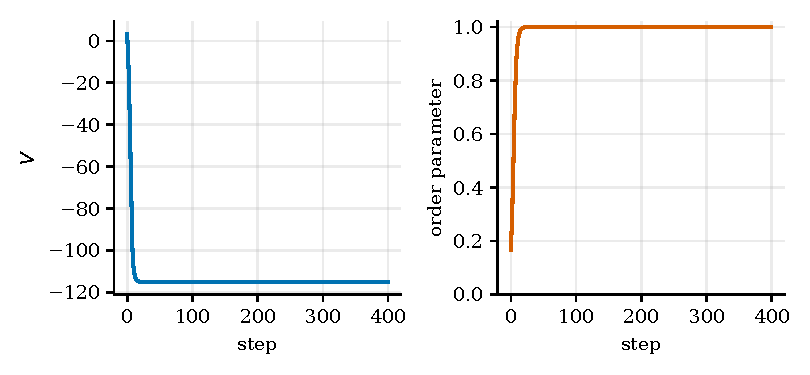
\includegraphics[width=0.85\textwidth]{figs/kuramoto}
\caption{Euler-discretized Kuramoto dynamics with $\omega_i=0$ on a random sparse symmetric coupling of 30 oscillators at step $0.9/\kappa$: the potential $V$ (decreasing at every step, as asserted) and the order parameter. Computed by the script \texttt{figs.py} with seed 8; an illustration of the stated analytic result and not an evaluation of the architecture.}\label{fig:kuramoto}
\end{figure}

\chapter{The Ecphoric Retrieval Engine}\label{ch:engine}

Retrieval is an iterative computation, and the specification must fix its initialization, its candidate activation, its refinement step, its convergence criterion, its confidence estimate, and its termination rule. The iteration is
\begin{equation}\label{eq:engine}
r^{(k+1)}=\mathcal T_\vartheta\bigl(r^{(k)},c,M,Z,\Theta^{(k)}\bigr),
\end{equation}
with the minimal instance $\mathcal T_\vartheta(r)=(1-\eta)r+\eta\sum_iw_im_i$ of Appendix~\ref{app:minimal}. The initial state is $r^{(0)}=c$, the cue projected into the content space, or $r^{(0)}=0$ if the cue is a pure context. Candidate activation computes the scores $s_i^{(k)}=R(m_i,U(z,\theta^{(k)})c)$ for a subset of traces selected by an index, exact in the baseline and approximate when Chapter~\ref{ch:budget} makes a budget binding. The refinement step is \eqref{eq:engine}, and convergence is declared when the residual $\norm{r^{(k+1)}-r^{(k)}}$ falls below a tolerance $\epsilon_{\mathrm{res}}$.

For a map known to be a $\lambda$-contraction, convergence has a certificate. If the residual at step $k$ is $\varrho_k=\norm{r^{(k)}-r^{(k-1)}}$, then Lemma~\ref{lem:banach} applied at the iterate gives the distance to the fixed point as at most $\lambda\varrho_k/(1-\lambda)$. The termination rule can therefore be stated in terms of a certified distance and not only in terms of a residual: stop when $\lambda\varrho_k/(1-\lambda)\le\epsilon$. For the damped softmax step with $\eta\in(0,1]$ and $\beta<1$, Theorem~\ref{thm:contract} gives the contraction factor $\lambda=1-\eta+\eta\beta$. The certificate is valid only for the fixed point it certifies, and by Example~\ref{ex:constant} it says nothing about whether that fixed point is the historically correct reconstruction.

Confidence estimation is therefore reported on two axes that must not be merged. The first is convergence confidence, the certified distance above. The second is selectivity, the information in the retrieval weights, which can be summarized by the entropy $H(w)$ or by the margin $\Delta=s_{(1)}-s_{(2)}$ between the largest and second largest scores. A sharp margin supports the claim that the output is close to one stored trace, by Proposition~\ref{prop:basin}. Neither axis measures fidelity, which requires the evidence-based statistics of Chapter~\ref{ch:reconsol}, and a conforming implementation must report the first two as properties of the computation and the third only when supporting evidence is available.

\section*{Executable specification of retrieval}\label{sec:retrievecode}

The retrieval engine of this chapter is specified by an iteration, and the lifecycle example at the end of Part~VIII uses its single-step form, so the form that is used is fixed here in pseudocode. The listing is a specification in the sense of Chapter~\ref{ch:refimpl}: it defines the interface and the invariants, it is deterministic given its inputs, and it is not a claim about performance.

\begin{figure}[t]
\centering
\begin{Verbatim}[fontsize=\footnotesize,frame=single,framesep=2mm]
RETRIEVE(M, L, c; beta, g, theta_d, tau)
  # M: traces m_1..m_P with ledger pointers nu_1..nu_P;  L: ledger;  c: cue
  1  for i in 1..P:  cos_i <- <m_i, c> / (|m_i| |c|)
  2  w <- softmax(beta * cos)
  3  F <- sum_i w_i m_i
  4  r <- (1 - g) F + g c                       # one cue-anchored step
  5  margin <- (largest cos) - (second largest cos)
  6  A <- { i : w_i >= tau }                    # attributed traces
  7  D <- { j : r_j >= theta_d }                # reportable details
  8  W <- { j in D : exists i in A with (m_i)_j >= 1/2 }   # warranted details
  9  omega <- |W| / |D|    (omega <- 1 if D is empty)
 10  append to L: interpretation(cue = c, cites = nu_i for i in A,
                                 weights = w, details = D)
 11  return (r, w, A, D, W, omega, margin)      # M is not modified
\end{Verbatim}
\caption{Single-step retrieval with attribution and warrant coverage. The traces are never modified by retrieval, and the only persistent effect is the appended interpretation record. The parameters used in the lifecycle example are $\beta=8$, $g=0.2$, $\theta_d=\tfrac14$ and $\tau=\tfrac12$.}\label{fig:retrievecode}
\end{figure}

Three properties of the listing are used below. Retrieval is a read-only operation on the store, so the persistent state after a retrieval differs from the state before it only by one ledger record. The warrant coverage $\omega$ of line 9 is computed from the stored traces and the attributed set $A$ and not from the reconstruction, so it can be low when the reconstruction is dominated by the cue; this is the separation between generative influence and warrant of Definition~\ref{def:warrant}. And the set $A$ may be empty, in which case $W$ is empty and $\omega=0$ for a nonempty $D$, which is how the specification reports that no single stored trace accounts for the answer.


\chapter{Persistent Memory and Historical Provenance}\label{ch:provenance}

The architecture must permit modification of a memory without silently rewriting the record of what was previously stored. The mechanism is an append-only ledger. A ledger is a set of typed records, each carrying an identifier, a type, a payload, a reference to the records it depends on, and a logical timestamp. Four record types are distinguished. An inscription records the original encoding of an observation: the content as first written, with the context and time. A transformation records a subsequent change to a trace, with the exact increment of Proposition~\ref{prop:reverse}. An interpretation records a reconstruction produced by the retrieval engine together with the cue and context that produced it, so that reconstructions are never confused with inscriptions. An evidence record records an observation that supports or contradicts a prior record and is the stated reason for any transformation that cites it. The pointer $\nu_i$ of a trace is the identifier of its latest record, and the full chain of records reachable from $\nu_i$ is the provenance of the trace.

A distinction that the ledger must support is between the evidence that generated a reconstruction and the evidence that warrants its historical attribution. A reconstruction can be causally influenced by a trace without that trace justifying every detail of the result: the weight a trace receives in the retrieval iteration measures its contribution to the computation, and says nothing about whether the inscription behind it entails a particular detail of the output, which may have been supplied by the context operator, by the cue, or by the blending of several traces. The two relations are recorded separately.

\begin{definition}[Generative influence and warrant]\label{def:warrant}
Let an interpretation record carry a reconstruction $r^\star$ with a set $A$ of separately reportable details. Its generative influence is the weight vector $w^{(K)}$ of the final refinement step, together with the sources of the cue and the context used. A detail $a\in A$ is warranted if there is an attributed trace, that is, a trace whose weight in $w^{(K)}$ is at least a declared attribution threshold $\tau_{\mathrm{attr}}$ (by default $\tfrac12$), such that the inscription record at the head of its citation chain, together with the logged transformations on that chain, determines the value of $a$ to within the stated tolerance under a declared entailment rule. The warrant coverage of the record is $\omega=|\{a\in A:a\text{ is warranted}\}|/|A|$, and the details outside the warranted set are labeled inferred.
\end{definition}

Warrant coverage is computed from the ledger and the entailment rule, independently of the retrieval weights, so a reconstruction with high generative influence from a trace and low warrant coverage is detected as one whose details were largely supplied by something other than the record. Source attribution in the sense of Chapter~\ref{ch:source} is a claim about warrant and not about influence, and the experiments of Chapter~\ref{ch:source-exp} measure it as such.

Three properties follow from the append-only discipline. The first is auditability: the chain from any trace to its inscription is available, and every transformation can be traced to its evidence. The second is reversibility, shown for logged increments in Proposition~\ref{prop:reverse}: any earlier state of a trace is recoverable from the current state and the ledger. The third is non-forgery: since interpretations are typed distinctly from inscriptions, a reconstruction cannot be mistaken for the original even if it is later promoted to a stored trace, because the promotion is itself a recorded transformation citing the interpretation as its source. This last property is what separates a system that has revised its memory from one that has lost track of its own history.

Deliberate forgetting is accommodated without breaking append-only semantics by tombstones. A tombstone is a record of type release that references the records it supersedes. Under the default policy of Chapter~\ref{ch:forgetting} the payloads of the superseded records are retained in cold storage so that the release is reversible; under an erasure policy the payloads are deleted and the tombstone records the fact and the time of deletion. In either case the ledger records that the release occurred, and what is lost under erasure is the content, never the knowledge that the content once existed. The relation between the ledger and the sufficiency criterion is direct: by the first qualification after Proposition~\ref{prop:identlimit}, a decoder that consults the ledger has the ledger as part of the memory state, and the sufficiency question is then asked of the combined encoding. This is the formal reason that source discrimination, which is impossible from content alone (Proposition~\ref{prop:source}), becomes possible when provenance is stored.


\begin{figure}[t]
\centering
\begin{tikzpicture}[>=Stealth,rec/.style={draw,rounded corners=2pt,minimum width=3.0cm,minimum height=.9cm,align=center,font=\small}]
\node[rec] (ins) at (0,0) {inscription\\observation $o$};
\node[rec] (tr) at (4.6,0) {transformation\\increment $\Delta_s$};
\node[rec] (rel) at (9.2,0) {release\\tombstone};
\node[rec] (int) at (0,-2.4) {interpretation\\reconstruction $r^\star$};
\node[rec] (ev) at (5.2,-2.4) {evidence\\supports or contradicts};
\draw[->] (tr) -- node[above,font=\scriptsize] {cites} (ins);
\draw[->] (rel) -- node[above,font=\scriptsize] {cites} (tr);
\draw[->] (ev) -- node[right,font=\scriptsize] {gates} (tr);
\draw[->] (int) -- node[left,font=\scriptsize] {cites} (ins);
\draw[->,dashed] (int) -- node[below,font=\scriptsize] {promoted} (ev);
\end{tikzpicture}
\caption{Typed records of the ledger and their citation structure. Arrows point from a record to the records it depends on; no record is removed, and a reconstruction can enter the store only through a transformation that cites it.}\label{fig:ledger}
\end{figure}

\section*{Executable specification of ledger replay}\label{sec:replaycode}

The derived state of Proposition~\ref{prop:derived} is computed by a fold, and the fold is the object that the replay requirement of the reference implementation tests.

\begin{figure}[t]
\centering
\begin{Verbatim}[fontsize=\footnotesize,frame=single,framesep=2mm]
REPLAY(L, init)
  # L: ledger records with Lamport timestamps;  init: payload -> initial vector
  1  M <- []                                  # list of traces, indexed by inscription
  2  for rec in L sorted by (counter, replica_id):
  3     if rec.type == inscription:
  4         append copy(init[rec.payload]) to M;  index[rec.id] <- len(M)
  5     if rec.type == transformation:
  6         i <- index of the trace cited first by rec
  7         M[i] <- M[i] + rec.payload          # logged increment, exact
  8     if rec.type == release:
  9         mark the trace cited by rec as released (payload kept in cold storage)
 10     # interpretation and evidence records do not change M
 11  return M
\end{Verbatim}
\caption{Deterministic derivation of the store from the ledger. The result depends only on the set of records, by Proposition~\ref{prop:derived}.}\label{fig:replaycode}
\end{figure}

A remark on arithmetic is needed, because Proposition~\ref{prop:reverse} is stated in real arithmetic and an implementation uses finite precision. Recovering an earlier state by subtracting later increments from the current state is exact in real arithmetic, but in floating point it can leave a rounding residue, since addition is not associative. The specification therefore recovers an earlier state by replaying the ledger up to the chosen time, and it uses subtraction only as an audit check. In the lifecycle example below all stored values and increments are dyadic rationals of small denominator, for which floating-point addition and subtraction are exact, so that both procedures agree bit for bit, and this is the reason those values were chosen. The choice is a device of the example; it does not make the property hold for arbitrary payloads.

Definition~\ref{def:warrant} counts a detail as warranted only through an attributed trace, and the lifecycle example shows why the threshold is needed. Under a softmax every trace has strictly positive weight, so if warrant required only positive generative influence then every detail present in any stored trace would be warranted and the coverage $\omega$ would be vacuous. The definition therefore requires the weight to reach $\tau_{\mathrm{attr}}$, a declared policy parameter, and takes the content of the trace to be its inscription together with its logged transformations, which is the form used by the listing of Figure~\ref{fig:retrievecode}.


\chapter{Adaptive Memory Organization}\label{ch:adaptive}

Five operations organize the store over time: consolidation, splitting, merging, abstraction, and forgetting. For each the specification must state an invariant for provenance, for accessibility, and for recoverability, and the invariants are the acceptance conditions for any implementation.

Consolidation transfers strength from the fast to the slow store by replay, with the dynamics of Proposition~\ref{prop:twostore}; its provenance invariant is that the slow-store trace carries the pointers of the fast-store traces it was built from, and its accessibility invariant is that the cue family supported before consolidation remains supported with at most the distortion allowed by the replay's learning rate. Splitting replaces a trace by two when a cue family is found to require a distinction that the trace blurs, such as when the same content has been associated with conflicting outcomes in different contexts; the provenance invariant is that both children cite the parent, and the recoverability invariant is that the parent is reconstructible from the pair, which holds exactly when the split is an additive decomposition $\psi=\psi'+\psi''$ and the ledger records the weights. Merging replaces a set of traces by one when they are redundant with respect to the committed cue family. Its admissibility is a corollary of Proposition~\ref{prop:distort}: merging two traces that differ by $\delta$ in norm replaces each by their mean, a displacement of $\delta/2$ per trace, so the readout changes by at most $(1+2\beta)\delta/2$ at every query in the unit ball, and the merge is admissible when this is below the tolerance $\varepsilon$ of the compression bound \eqref{eq:compbound}. Abstraction creates a trace representing a class by the mean of its members, retaining the members in the ledger; it is the operation by which the slow store acquires semantic structure, and its admissibility is the closure criterion of Proposition~\ref{prop:closure} for the projection that sends members to the class. Forgetting follows Chapter~\ref{ch:forgetting} and always leaves a tombstone.

\begin{proposition}[Provenance is preserved by every organizing operation]\label{prop:provinv}
Suppose each of the five operations is implemented as an append of new records that reference the records they act on, and never as a modification or deletion of an existing record, except that erasure policy may delete payloads of released records. Then for every trace present at any time, the chain from its pointer to the inscriptions of the observations it derives from is complete, and the set of records only grows.
\end{proposition}

\begin{proof}
Each operation appends records that cite their inputs, so by induction on the number of operations every trace's chain reaches inscriptions through citations that are never removed. The set of records grows monotonically because no operation removes a record, and erasure removes only payloads, which does not alter the citation structure.
\end{proof}

\section*{Executable specification of controlled reconsolidation and a merge check}\label{sec:reconcode}

The evidence-gated update of Chapter~\ref{ch:reconsol} and the provenance invariant of Proposition~\ref{prop:provinv} fix what a revision must do, and the listing below fixes how.

\begin{figure}[t]
\centering
\begin{Verbatim}[fontsize=\footnotesize,frame=single,framesep=2mm]
RECONSOLIDATE(M, L, i, e, reports; eta, Lambda_star)
  # i: trace to revise;  e: evidence-bearing target;  reports: {(source, rho)}
  1  keep one report per distinct source          # no double counting
  2  Lambda <- product over kept reports of rho / (1 - rho)
  3  ev <- append to L: evidence(cites = nu_i, payload = reports)
  4  if Lambda < Lambda_star:  return M           # gate closed, store unchanged
  5  Delta <- eta * (e - m_i)                      # exact increment
  6  tr <- append to L: transformation(cites = nu_i and ev, payload = Delta)
  7  m_i <- m_i + Delta;  nu_i <- tr
  8  return M

REVERSE(M, L, i, tr)
  1  Delta <- payload of tr
  2  tr' <- append to L: transformation(cites = nu_i and tr, payload = -Delta)
  3  m_i <- m_i - Delta;  nu_i <- tr'              # nothing is deleted
\end{Verbatim}
\caption{Evidence-gated revision and its reversal. The evidence record is appended whether or not the gate opens, so that the rejected evidence remains auditable. Reversal appends an inverse increment and does not remove records.}\label{fig:reconcode}
\end{figure}

By construction every operation in the listing appends and none removes, so the hypothesis of Proposition~\ref{prop:provinv} holds, and by Proposition~\ref{prop:derived} the store after any sequence of operations equals the replay of its ledger. The gate of line 4 aggregates by source, which is the discipline that Counterexample~\ref{cex:gate28} shows to be necessary.

\begin{workedex}[Admissibility of a merge]\label{ex:merge42}
Merging two traces at distance $d$ into their midpoint moves each by $d/2$, so by Proposition~\ref{prop:distort} the readout of any cue changes by at most $(1+2\beta)d/2$. A merge is therefore admissible for a compression budget $\varepsilon$ if $d\le2\varepsilon/(1+2\beta)$. For $\beta=8$ and $\varepsilon=0.05$ the threshold is $d\le\ndmax$, a very small distance, which shows that at selective temperatures only near-identical traces can be merged on the strength of this sufficient condition alone. In 300 random stores with a planted near-duplicate pair, the largest observed ratio of the actual readout change to the bound $(1+2\beta)d/2$ was $\nmergeratio$. The bound was therefore never violated and was loose by a factor of about thirty-seven on those stores. Because Extension~\ref{ext:sharp30} shows that the dependence on $\beta$ cannot be improved in general, a larger threshold must come from structural knowledge of the cue family, which is what the quotient of Extension~\ref{ext:viabequiv} provides. These are algebraic checks of the proposition with a fixed seed and not measurements on a memory.
\end{workedex}


\paragraph{A unified learning objective.} The operations above are mechanisms, and a trainable architecture needs a single objective that couples them. Let $\vartheta$ collect the continuous parameters of the representation (the encoder of content and the context operator $U$), of the oscillatory engine ($\omega$, $K$), and of the retrieval engine ($\beta$, $\eta$, any gating maps), and let the discrete operations (merging, splitting, release) be governed by rules whose thresholds are hyperparameters. Over streams of episodes and cues with targets $T$, the learning problem is
\begin{equation}\label{eq:learnobj}
\min_{\vartheta}\ \Ex\Bigl[\sum_t\ell\bigl(r^\star_t(\vartheta),T(h_t,c_t)\bigr)+\lambda\,C_t(\vartheta)\Bigr]\quad\text{subject to}\quad\Ex[D_t]\le\delta\ \text{and}\ X_t\in\Viab(K)\ \ \text{for all }t,
\end{equation}
where $\ell$ is the reconstruction loss, $C_t$ the computational cost, $D_t$ the fidelity distortion of Chapter~\ref{ch:viability}, and the second constraint confines the discrete operations to the viability kernel. The constraints are handled by a Lagrangian with a multiplier on the fidelity term updated by dual ascent, which converges to a solution that respects the constraint and, unlike a fixed penalty, does not depend on the scale of the loss (Proposition~\ref{prop:penalty}). The retrieval engine is differentiable in $\vartheta$ whenever it is a contraction, which makes the objective trainable without backpropagating through the unrolled iteration.

\begin{proposition}[Implicit differentiation through a contractive retrieval]\label{prop:implicit}
Let $F(r;\vartheta)$ be continuously differentiable jointly in $(r,\vartheta)$ with $\norm{\partial_rF}\le\lambda<1$ and $\norm{\partial_\vartheta F}\le L_\vartheta$. Then the fixed point $r^\star(\vartheta)$ is continuously differentiable and
\begin{equation}
\frac{\partial r^\star}{\partial\vartheta}=\bigl(I-\partial_rF\bigr)^{-1}\partial_\vartheta F\Big|_{r^\star},\qquad\Bigl\|\frac{\partial r^\star}{\partial\vartheta}\Bigr\|\le\frac{L_\vartheta}{1-\lambda}.
\end{equation}
\end{proposition}

\begin{proof}
Since $\norm{\partial_rF}<1$, the matrix $I-\partial_rF$ is invertible with $\norm{(I-\partial_rF)^{-1}}\le1/(1-\lambda)$ by the Neumann series. The implicit function theorem applied to $r-F(r;\vartheta)=0$ gives differentiability and the formula, and the bound follows.
\end{proof}

The learning problem \eqref{eq:learnobj} makes the relation among consolidation, reconsolidation and the representation explicit: they are components of one constrained optimization, in which consolidation shapes the targets that the loss measures, evidence-gated reconsolidation changes the targets $T$ only through recorded evidence, and the representation and oscillator parameters are learned against the resulting stream. The specification does not claim that the optimization has been carried out; it states what the training problem is, so that the experiments of Part~IX have a defined object to train.

\chapter{Resource Scheduling and Bounded Computation}\label{ch:budget}

The ideal system of Part~VII has no resource limits, and the practical system has a budget $B_t$ on time, memory and energy. The scheduler decides, for each retrieval, how many refinement steps to spend, how many traces to activate, and whether to attempt reconstruction at all. The central quantity is the marginal value of a further step, which for a contractive refinement can be stated exactly.

Suppose the iteration is a $\lambda$-contraction with initial certified error $R$ and that each step costs $\varsigma>0$ in the units of the objective, with the penalty for remaining error equal to the error itself. The total cost after $k$ steps is bounded by
\begin{equation}\label{eq:budgetcost}
J(k)=R\lambda^k+\varsigma k,
\end{equation}
where the first term is the error bound of Lemma~\ref{lem:banach}.

\begin{proposition}[Optimal stopping for contractive refinement]\label{prop:stopping}
The function $J$ is convex in $k$ and its continuous minimizer is
\begin{equation}
k^\star=\frac{1}{\ln(1/\lambda)}\ln\!\Bigl(\frac{R\ln(1/\lambda)}{\varsigma}\Bigr)
\end{equation}
when $R\ln(1/\lambda)>\varsigma$, and $J$ is minimized at $k=0$ otherwise. The integer minimizer is $\lfloor k^\star\rfloor$ or $\lceil k^\star\rceil$.
\end{proposition}

\begin{proof}
$J''(k)=R(\ln\lambda)^2\lambda^k>0$, so $J$ is convex. Setting $J'(k)=-R\ln(1/\lambda)\lambda^k+\varsigma=0$ gives $\lambda^k=\varsigma/(R\ln(1/\lambda))$, hence $k^\star$. If $R\ln(1/\lambda)\le\varsigma$ then $J'(0)\ge0$ and convexity gives the minimum at zero. For a convex function on the integers the minimizer is one of the two integers adjacent to the continuous minimizer.
\end{proof}

The proposition formalizes the rule that further reconstruction is worth its cost until the marginal reduction of the error bound falls to the marginal cost of a step, and it shows that slow contractions (with $\lambda$ near one) justify a number of steps that grows like $1/\ln(1/\lambda)$. It also identifies the failure mode of a fixed iteration count: an easy cue, with a small $R$, wastes steps, and a hard cue is stopped before the bound is useful.

Graceful degradation under a binding budget has a specification. The retrieval engine reduces cost in a fixed order, first by shortening the refinement, then by restricting activation to the top-$K$ traces by a cheap prefilter, then by lowering the precision of the scores, and only then by declining to answer. At every stage the response reports the residual certificate and the margin of Chapter~\ref{ch:engine}, so that the downstream consumer can tell a reduced-effort answer from a full-effort one. Critical historical distinctions are protected by marking traces whose release or merge would leave the viability kernel of Chapter~\ref{ch:viability}; the scheduler never prefilters them out and never merges them, whatever the budget, which makes this a hard constraint and not a penalty.

Figure~\ref{fig:stopping} shows the trade-off of Proposition~\ref{prop:stopping}: the error bound falls geometrically while cost grows linearly, and the optimum sits where their slopes cancel.

\begin{figure}[t]
\centering
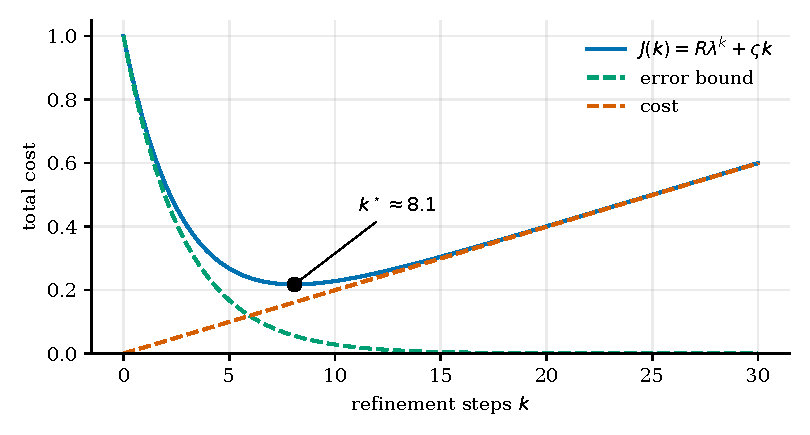
\includegraphics[width=0.85\textwidth]{figs/stopping}
\caption{Total cost $J(k)=R\lambda^k+\varsigma k$ with $R=1$, $\lambda=0.7$, $\varsigma=0.02$, and its minimizer from Proposition~\ref{prop:stopping}. Computed by the script \texttt{figs.py} with seed 8; an illustration of the stated analytic result and not an evaluation of the architecture.}\label{fig:stopping}
\end{figure}

\begin{workedex}[Easy and hard cues under a fixed iteration count]\label{ex:stop43}
Take $\lambda=0.7$ and a step cost $\varsigma=0.02$. For the certified initial error $R=1$ the optimal stopping index is $k^\ast=\nkstar$, the integer optimum is $k=\nkint$ with cost $J(8)=\nJint$, and doing nothing costs $J(0)=\nJA$ while a fixed count of twenty steps costs $J(20)=\nJCA$, nearly twice the optimum. For an easy cue with $R=0.05$ one has $R\ln(1/\lambda)=0.018<\varsigma$, so Proposition~\ref{prop:stopping} says to take no step, at cost $\neasyJA$, and a fixed count of eight would cost $\neasyfixed$, which is $\neasyratio$ times as much. For a hard cue with $R=5$ the optimum is $k^\ast=\nhardk$, the integer minimizer is $\nhardkint$ with cost $\nhardJopt$, and stopping at the fixed count of eight costs $\nhardfixed$, a factor $\nhardratio$ above the optimum. The same fixed count is thus too long for one cue and too short for the other, which is the failure mode that the certified residual is meant to remove. These costs are computed from the formula $J(k)=R\lambda^k+\varsigma k$ and do not describe a measured system.
\end{workedex}


\chapter{Distributed and Asynchronous Memory}\label{ch:distributed}

Several nodes may hold replicas of a memory and update them concurrently, with delayed observations and temporarily inconsistent local histories. The architecture requires eventual reconciliation without loss of any node's inscriptions. The ledger of Chapter~\ref{ch:provenance} provides the natural structure, since a set of records with set union as the merge operation has the algebra needed.

\begin{proposition}[Convergence of ledger replicas]\label{prop:crdt}
Let each replica hold a set of records, grow it by adding records, and merge by set union. Then merge is commutative, associative and idempotent, so any two replicas that have received the same set of records, in any order and with any duplication, hold the same set. Equivalently, the replica states form a join-semilattice under inclusion, and every replica's state is monotone under updates and merges.
\end{proposition}

\begin{proof}
Union is commutative, associative and idempotent. Two replicas that have received the same collection of records, however ordered and duplicated, hold the union of that collection, which is a single set.
\end{proof}

Agreement on the set of records is not yet agreement on the derived memory state, because transformations may not commute: applying an increment $\Delta_1$ followed by a gated update is different from the reverse. The derived state is therefore defined as a fold of the update function over the records in a canonical total order. Give every record a Lamport timestamp \cite{lamport1978} $(\ell,\mathrm{id})$ consisting of a logical counter and the identifier of the originating replica; the lexicographic order on pairs is total, is consistent with causality, and is the same at every replica.

\begin{proposition}[Deterministic derived state]\label{prop:derived}
If the update function is deterministic and records are folded in the order of their timestamps $(\ell,\mathrm{id})$, then any two replicas holding the same set of records compute the same memory state. Late-arriving records with earlier timestamps are accommodated by replaying from the first affected position.
\end{proposition}

\begin{proof}
The timestamp order is a total order on the common set, so the fold is the same sequence of applications at both replicas, and a deterministic update function yields the same result. A late record changes the sequence only from its own position onward, so replaying from that position reproduces the fold.
\end{proof}

The proposition is the formal basis for the replay requirement of the reference implementation. Its cost is the replay length, and the obvious engineering response is periodic snapshots, which are caches of derived state and not memory state, and are discarded when a late record invalidates them. Where updates commute, as with additive increments, the order is immaterial and replay can be avoided entirely.

The distinction between shared semantic knowledge and independently acquired episodic evidence has a precise form in this setting. Semantic content, the slow-store abstractions of Chapter~\ref{ch:adaptive}, is replicated and reconciled by consolidating the union of the nodes' episodic records, and it is an output of the fold. Episodic evidence is never overwritten by another node's semantic abstraction; it is a record in the ledger with the identifier of the node that observed it. A node that receives a conflicting abstraction can compare it with its own episodic records, which is the mechanism by which inconsistent local histories are detected and not merely overwritten.

\begin{workedex}[Non-commuting updates at two replicas]\label{ex:replica44}
Let the memory state be a single number $s$ with initial value $1$. Replica $A$ produces the record $a=(\ell{=}1,A,\text{scale by }2)$ and replica $B$ the record $b=(\ell{=}1,B,\text{add }3)$ concurrently. If a replica applies records in the order of arrival, the node that receives $a$ first computes $1\cdot2+3=\nrepAB$ and the node that receives $b$ first computes $(1+3)\cdot2=\nrepBA$, so two replicas that hold the same set of records disagree on the state, although Proposition~\ref{prop:crdt} guarantees that they agree on the set. Folding in the Lamport order $(\ell,\mathrm{id})$ places $a$ before $b$ at both replicas and gives $\nrepAB$ at each. Suppose now a record $c=(\ell{=}0,C,\text{add }10)$ from a third replica arrives late. The canonical order is $c,a,b$, and replaying from the first affected position gives $((1+10)\cdot2)+3=\nreplate$ at every replica, whatever order the three records were received in, which is the statement of Proposition~\ref{prop:derived}. Where updates commute, as for additive increments, the arrival order would have sufficed and replay could be skipped, which is the cost saving noted after the proposition.
\end{workedex}


\chapter{Reference Implementation}\label{ch:refimpl}

The reference implementation is organized as six modules whose interfaces are fixed so that each can be replaced independently: the representation (encoding and decoding of the trace tuple), the resonance scorer $R$, the oscillator $\mathfrak C$ of Chapter~\ref{ch:oscengine}, the ecphoric reconstruction engine of Chapter~\ref{ch:engine}, the provenance store of Chapter~\ref{ch:provenance}, and the evaluation harness. Replaceability is not a convenience; it is what makes the ablation experiments of Part~IX meaningful, because an ablation changes exactly one module and holds the others fixed.


\begin{figure}[t]
\centering
\begin{tikzpicture}[>=Stealth,box/.style={draw,rounded corners=2pt,minimum width=3.0cm,minimum height=.95cm,align=center,font=\small}]
\node[box] (cue) at (0,0) {cue $c$\\context $Z$};
\node[box] (osc) at (4.3,0) {oscillator\\$\mathfrak C$};
\node[box] (score) at (8.6,0) {scorer $R$\\weights $w^{(k)}$};
\node[box] (out) at (0,-2.3) {reconstruction $r^\star$\\certificate, margin};
\node[box] (eng) at (4.3,-2.3) {retrieval engine\\$r^{(k+1)}=\mathcal T_\vartheta(\cdot)$};
\node[box] (mem) at (8.6,-2.3) {persistent traces\\$M$};
\node[box] (led) at (4.3,-4.6) {ledger\\(append only)};
\draw[->] (cue) -- (osc);
\draw[->] (osc) -- node[above,font=\scriptsize] {$\Phi^{(k)}$} (score);
\draw[->] (mem) -- (score);
\draw[->] (score.south west) -- (eng.north east);
\draw[->] (eng) -- (out);
\draw[->] (eng) -- node[right,font=\scriptsize] {interpretation record} (led);
\draw[->] (led.east) -| node[below right,font=\scriptsize,pos=.2] {$\nu_i$} (mem.south);
\draw[->,dashed] (eng.north) -- node[left,font=\scriptsize,pos=.4] {$r^{(k)}$} (osc.south);
\end{tikzpicture}
\caption{Module structure of the reference implementation. Each box is an independently replaceable module; the dashed arrow is the feedback of the current reconstruction into the context operator and the scores, absent in the minimal model of Appendix~\ref{app:minimal}.}\label{fig:modules}
\end{figure}

Three engineering requirements are binding. The first is determinism: with fixed seeds and a fixed order of events the implementation must produce bit-identical memory states, so that Proposition~\ref{prop:derived} is realized in code and any discrepancy is a defect. The second is instrumentation: every retrieval emits the cue, the context, the scores, the weights, the iterates, the residual certificates and the final reconstruction to an interpretation record, so that nothing about a reconstruction is discoverable only by rerunning it. The third is replay: any memory transition can be reproduced from the ledger and the seed, and the test suite includes a replay check that rebuilds the state from the ledger and compares it with the live state.

The minimal model of Appendix~\ref{app:minimal} is the first conforming instance. Its deliberately limited scope should be stated: it has no learning rules, no temporal sequence representation, no uncertainty beyond the retrieval weights, and no persistent-state updates, and the modules above are specified so that each of these can be added without changing the others. The pilot calculations of Appendix~\ref{app:pilot} check the algebraic claims of Parts~II and III in this setting and do not constitute an evaluation of the architecture.

\section*{A complete miniature memory lifecycle}\label{sec:lifecycle}

The components of Part~VIII are exercised together by a deterministic walk through one memory from encoding to revision and audit. The setting is deliberately tiny so that every number can be inspected: seven binary features (\emph{Ann}, \emph{Bo}, \emph{cafe}, \emph{library}, \emph{rain}, \emph{morning}, \emph{evening}), three episodes $E_1=(\emph{Ann},\emph{cafe},\emph{morning})$, $E_2=(\emph{Ann},\emph{library},\emph{rain})$ and $E_3=(\emph{Bo},\emph{cafe},\emph{rain})$, and the parameters $\beta=8$, $g=0.2$, $\theta_d=\tfrac14$, $\tau_{\mathrm{attr}}=\tfrac12$ and $\Lambda^\ast=10$. The procedures are those of Figures~\ref{fig:retrievecode}, \ref{fig:replaycode} and~\ref{fig:reconcode}. The script \texttt{lifecycle.py} carries out every step with exact arithmetic and asserts, after every operation, that the ledger has only grown and that replaying it reproduces the store. The walk is an illustration of the specification on invented data and is not an empirical finding.

\begin{table}[p]
\centering
\small
\renewcommand{\arraystretch}{1.2}
\begin{tabular}{@{}l p{3.0cm} p{5.2cm} p{2.6cm}@{}}
\toprule
Step & Operation & Persistent traces after the operation & Ledger records \\
\midrule
S0 & empty store & \footnotesize (empty) & \footnotesize none \tabularnewline
S1 & encode E1 & \footnotesize $m_1=(1,0,1,0,0,1,0)$ & \footnotesize 1i \tabularnewline
S2 & encode E2, E3 & \footnotesize $m_1=(1,0,1,0,0,1,0)$\par $m_2=(1,0,0,1,1,0,0)$\par $m_3=(0,1,1,0,1,0,0)$ & \footnotesize 1i 2i 3i \tabularnewline
S3 & partial cue (Ann, morning) & \footnotesize $m_1=(1,0,1,0,0,1,0)$\par $m_2=(1,0,0,1,1,0,0)$\par $m_3=(0,1,1,0,1,0,0)$ & \footnotesize 1i 2i 3i 4p \tabularnewline
S4 & misleading cue (adds rain) & \footnotesize $m_1=(1,0,1,0,0,1,0)$\par $m_2=(1,0,0,1,1,0,0)$\par $m_3=(0,1,1,0,1,0,0)$ & \footnotesize 1i 2i 3i 4p 5p \tabularnewline
S5 & misleading report, gate closed & \footnotesize $m_1=(1,0,1,0,0,1,0)$\par $m_2=(1,0,0,1,1,0,0)$\par $m_3=(0,1,1,0,1,0,0)$ & \footnotesize 1i 2i 3i 4p 5p 6e \tabularnewline
S6 & corroborated evidence, revise m1 & \footnotesize $m_1=(1,0,1,0,0,0,1)$\par $m_2=(1,0,0,1,1,0,0)$\par $m_3=(0,1,1,0,1,0,0)$ & \footnotesize 1i 2i 3i 4p 5p 6e 7e 8t \tabularnewline
S7 & later recollection (Ann, evening) & \footnotesize $m_1=(1,0,1,0,0,0,1)$\par $m_2=(1,0,0,1,1,0,0)$\par $m_3=(0,1,1,0,1,0,0)$ & \footnotesize 1i 2i 3i 4p 5p 6e 7e 8t 9p \tabularnewline
S8 & replay from ledger (state identical) & \footnotesize $m_1=(1,0,1,0,0,0,1)$\par $m_2=(1,0,0,1,1,0,0)$\par $m_3=(0,1,1,0,1,0,0)$ & \footnotesize 1i 2i 3i 4p 5p 6e 7e 8t 9p \tabularnewline
S9 & audit: rewind 8t, read only (store unchanged) & \footnotesize $m_1=(1,0,1,0,0,0,1)$\par $m_2=(1,0,0,1,1,0,0)$\par $m_3=(0,1,1,0,1,0,0)$ & \footnotesize 1i 2i 3i 4p 5p 6e 7e 8t 9p \tabularnewline
S10 & reverse revision: append inverse transformation & \footnotesize $m_1=(1,0,1,0,0,1,0)$\par $m_2=(1,0,0,1,1,0,0)$\par $m_3=(0,1,1,0,1,0,0)$ & \footnotesize 1i 2i 3i 4p 5p 6e 7e 8t 9p 10t \tabularnewline
\bottomrule

\end{tabular}
\caption{The persistent state after every operation of the lifecycle. Ledger records are numbered in order of creation and suffixed by type: i inscription, p interpretation, e evidence, t transformation. Retrieval steps change only the ledger, and the only steps that change a trace are S6 and S10.}\label{tab:lifecycle}
\end{table}

\paragraph{Encoding and partial-cue reconstruction (S1 to S3).} Encoding the three episodes appends three inscriptions and creates three traces. The cue $(\emph{Ann},\emph{morning})$ is partial, since it does not mention the place. Retrieval gives weight $\nwA$ to the first trace and $\nwAtwo$ to the second, with a cosine margin of $\nmarginA$ between the best and the second best trace, so the first trace is the single attributed trace. The reconstruction contains the details \emph{Ann}, \emph{cafe} and \emph{morning}; the cafe is supplied by the stored trace and not by the cue, and it is warranted by that trace, so the warrant coverage is $\nomegaA$. The store is unchanged and the ledger gains an interpretation record, 4p.

\paragraph{Misleading cue (S4).} The cue $(\emph{Ann},\emph{cafe},\emph{morning},\emph{rain})$ adds a feature that episode $E_1$ does not contain. The first trace still receives weight $\nwB$ and is attributed, but the reconstruction now reports \emph{rain} among its details, with component $\nrainB$ in the reconstructed vector, supplied by the cue and by the other traces and not by the attributed one. Warrant coverage is $\nomegaB$, three of the four details, and the report labels \emph{rain} as inferred. The example also shows the danger that Proposition~\ref{prop:drift} describes. If the reconstruction were written back to the first trace with rate $\tfrac12$ and no evidence, the trace would move by $\nhypshift$ in norm and acquire a rain component of $\nhyprain$ that no observation supports. The specification does not do this; the store is unchanged and the ledger gains 5p.

\paragraph{Misleading and then corroborating evidence (S5 and S6).} A single report that the episode took place at the library, from a source of reliability $0.6$, has likelihood ratio $\nlamone$ and the gate stays closed at $\Lambda^\ast=10$. The evidence is nonetheless recorded (6e), so the rejected report remains auditable. Three reports from three distinct sources, each of reliability $0.7$ and each saying that the episode was in the evening, give $\Lambda=\nlamthree$ and the gate opens. The revision moves the first trace by the increment $\Delta=e-m_1$ with $e=(\emph{Ann},\emph{cafe},\emph{evening})$, which flips the morning and evening features and moves the trace by $\nLdist$ in norm. The ledger gains the evidence record 7e and the transformation 8t, which cites the inscription 1i and the evidence 7e. The one-vote-per-source rule of Figure~\ref{fig:reconcode} matters here, since three copies of one report would have given only $\Lambda=\nlamcopy$ (Counterexample~\ref{cex:gate28}).

\paragraph{Later recollection (S7).} The cue $(\emph{Ann},\emph{evening})$ now attributes weight $\nwC$ to the revised trace and returns warrant coverage $\nomegaC$ with an interpretation record that cites the transformation 8t. The revision also changes how the original cue behaves: the cue $(\emph{Ann},\emph{morning})$, which gave weight $\nwA$ before the revision, gives only $\nwOldCue$ afterwards, below the attribution threshold, so no single trace is attributed to it and the specification reports that no trace accounts for the answer. This is the intended consequence of a justified revision and not an error.

\paragraph{Replay, audit and reversal (S8 to S10).} Replaying the ledger from the inscriptions reproduces the store exactly (S8). Subtracting the logged increment from the current state recovers the state at S5, so the audit of S9 changes nothing. Reversal (S10) appends an inverse transformation citing 8t, which returns the first trace to its original value while the ledger grows to $\nnledger$ records, none deleted, and a second replay again reproduces the store. The history of the memory therefore contains the revision and its undoing, and both remain open to inspection.

\begin{extension}[Lifecycle invariants]\label{ext:lifecycle}
Let the operations of Figures~\ref{fig:retrievecode}, \ref{fig:replaycode} and~\ref{fig:reconcode}, together with encoding, be applied in any order with the one-vote-per-source rule and exact arithmetic. Then after every operation (i) the record set is a superset of the record set before it, (ii) $\mathrm{REPLAY}(L)=M$, and (iii) a retrieval leaves $M$ unchanged. The first two are Propositions~\ref{prop:provinv} and~\ref{prop:derived} applied to this operation set, and the third is read off line 11 of Figure~\ref{fig:retrievecode}.
\end{extension}

The extension is a restatement and is included because the lifecycle verifies it at every step of one trajectory, which is evidence that the specification is consistent, and no more than that. It says nothing about whether the revisions are correct, since correctness depends on the evidence, and the evidence in the example was constructed.

\section*{Synthesis of Part~VIII}\label{sec:synth8}

The architecture of Part~VIII can be summarized by one rule and the checks that enforce it: nothing that has been written is removed, and every state is a function of the record set. The retrieval listing returns a reconstruction together with the attribution and warrant that justify it, and leaves the store alone (Figure~\ref{fig:retrievecode}). The reconsolidation listing admits a change to a trace only when evidence aggregated over distinct sources passes the gate, and it logs both the evidence and the increment (Figure~\ref{fig:reconcode}). The replay listing derives the store from the record set in a canonical order, which is what makes replicas that hold the same records agree even when their updates do not commute (Worked Example~\ref{ex:replica44}). The lifecycle ties these together: the misleading cue, the single report and the three reports exercise the three failure modes that the earlier parts identified, namely self-reinforcing distortion (Proposition~\ref{prop:drift}), uncorroborated revision, and double counting of evidence (Counterexample~\ref{cex:gate28}).

The links to the earlier parts are as follows. The sufficiency criterion of Part~VII applies to the combined encoding of store and ledger, by the first qualification after Proposition~\ref{prop:identlimit}, so the ledger is what allows a decoder to report that a detail is inferred, that a trace is no longer attributed to a cue, or that a state existed before a revision; none of these answers is available from the store alone. The quotient of Extension~\ref{ext:viabequiv} determines which traces may be merged or released without leaving the viable set, and the merge check of Worked Example~\ref{ex:merge42} is the conservative version of that determination in the absence of structural knowledge. The scheduling of Chapter~\ref{ch:budget} acts on the retrieval of Figure~\ref{fig:retrievecode}, and Worked Example~\ref{ex:stop43} shows that its stopping rule depends on the certified error of the cue and not on a count. The rates and thresholds of Part~VI enter through $\eta$, $\Lambda^\ast$ and $\beta$.

What the part does not establish is performance. The examples are exact computations on invented data chosen to display the logic of the specification, and the experimental protocols of Part~IX remain protocols. The pilot appendix lists the scripts \texttt{examples.py} and \texttt{lifecycle.py} that produced every number in Parts~VI to VIII, so that a reader can rerun them and obtain the same values.
